%% LaTeX2e class for student theses
%% sections/methodology.tex
%% 
%% Karlsruhe Institute of Technology
%% Institute for Program Structures and Data Organization
%% Chair for Software Design and Quality (SDQ)
%%
%% Dr.-Ing. Erik Burger
%% burger@kit.edu
%%
%% Version 1.3.2, 2017-08-01

\chapter{Methodology}
\label{ch:Methodology}
The approach to developing an automatic system to detect procedures administered by EMS personnel consists of breaking the procedures into anatomical movements, developing an algorithm, and collecting data to train a machine learning model through a user study. EMS personnel perform various procedures inside an ambulance. This thesis focuses on automatically detecting five procedures: placing a intravenous tourniquet, wrapping a wound, applying a bag-valve-mask, placing an oral airway, and \gls{CPR}. The five EMS procedures were chosen for their reproducibility on a demo mannequin.

\section{Hierarchical Task Analysis}
\label{sec:Approach:Hierarchical-Task-Analysis}
 Five procedures were picked for their assumed recognition difficulty. CPR is assumed to be easily recognizable, due to the repetitive motion during compressions in the accelerometer data. Bag-valve-mask application is assumed to be easily recognizable, due to the repetitive motion during squeezing the bag in the EMG data. Placing a tourniquet is assumed to be harder to recognize, due to missing repetitive motion. Wrapping a wound is assumed to be harder to recognize, due to missing repetitive motion. Placing an oral airway is assumed to be the hardest to recognize, due to missing repetitive motion and a short duration. Medical procedures include repetitive and unique movements. Machine-learning algorithms achieve higher performance when there are distinctive patterns in the data. Therefore, the EMS procedures are broken into their atomical movements using \emph{Hierarchical Task Analysis} in order to identify distinctive patterns in the EMS procedures \cite{kirwan1992guide}. The resulting anatomical movements are analyzed to include their sensability using commercially available sensors: Apple Watch, Myo, Empatic E4, Garmin Watch Forerunner, and Bioharness BT. The sensability is useful to determine what sensor to use to detect the anatomical movements. The analysis is done by considering the type of sensor data and their ability to detect anatomical movements, such as recognizing muscle movement through EMG data. The placement of a sensor is crucial in its ability to detect anatomical movements. The anatomical movements were verified by talking to EMS personnel at a local fire station.
\begin{figure}
 	\centering
 	\begin{subfigure}[b]{0.18\textwidth}
 		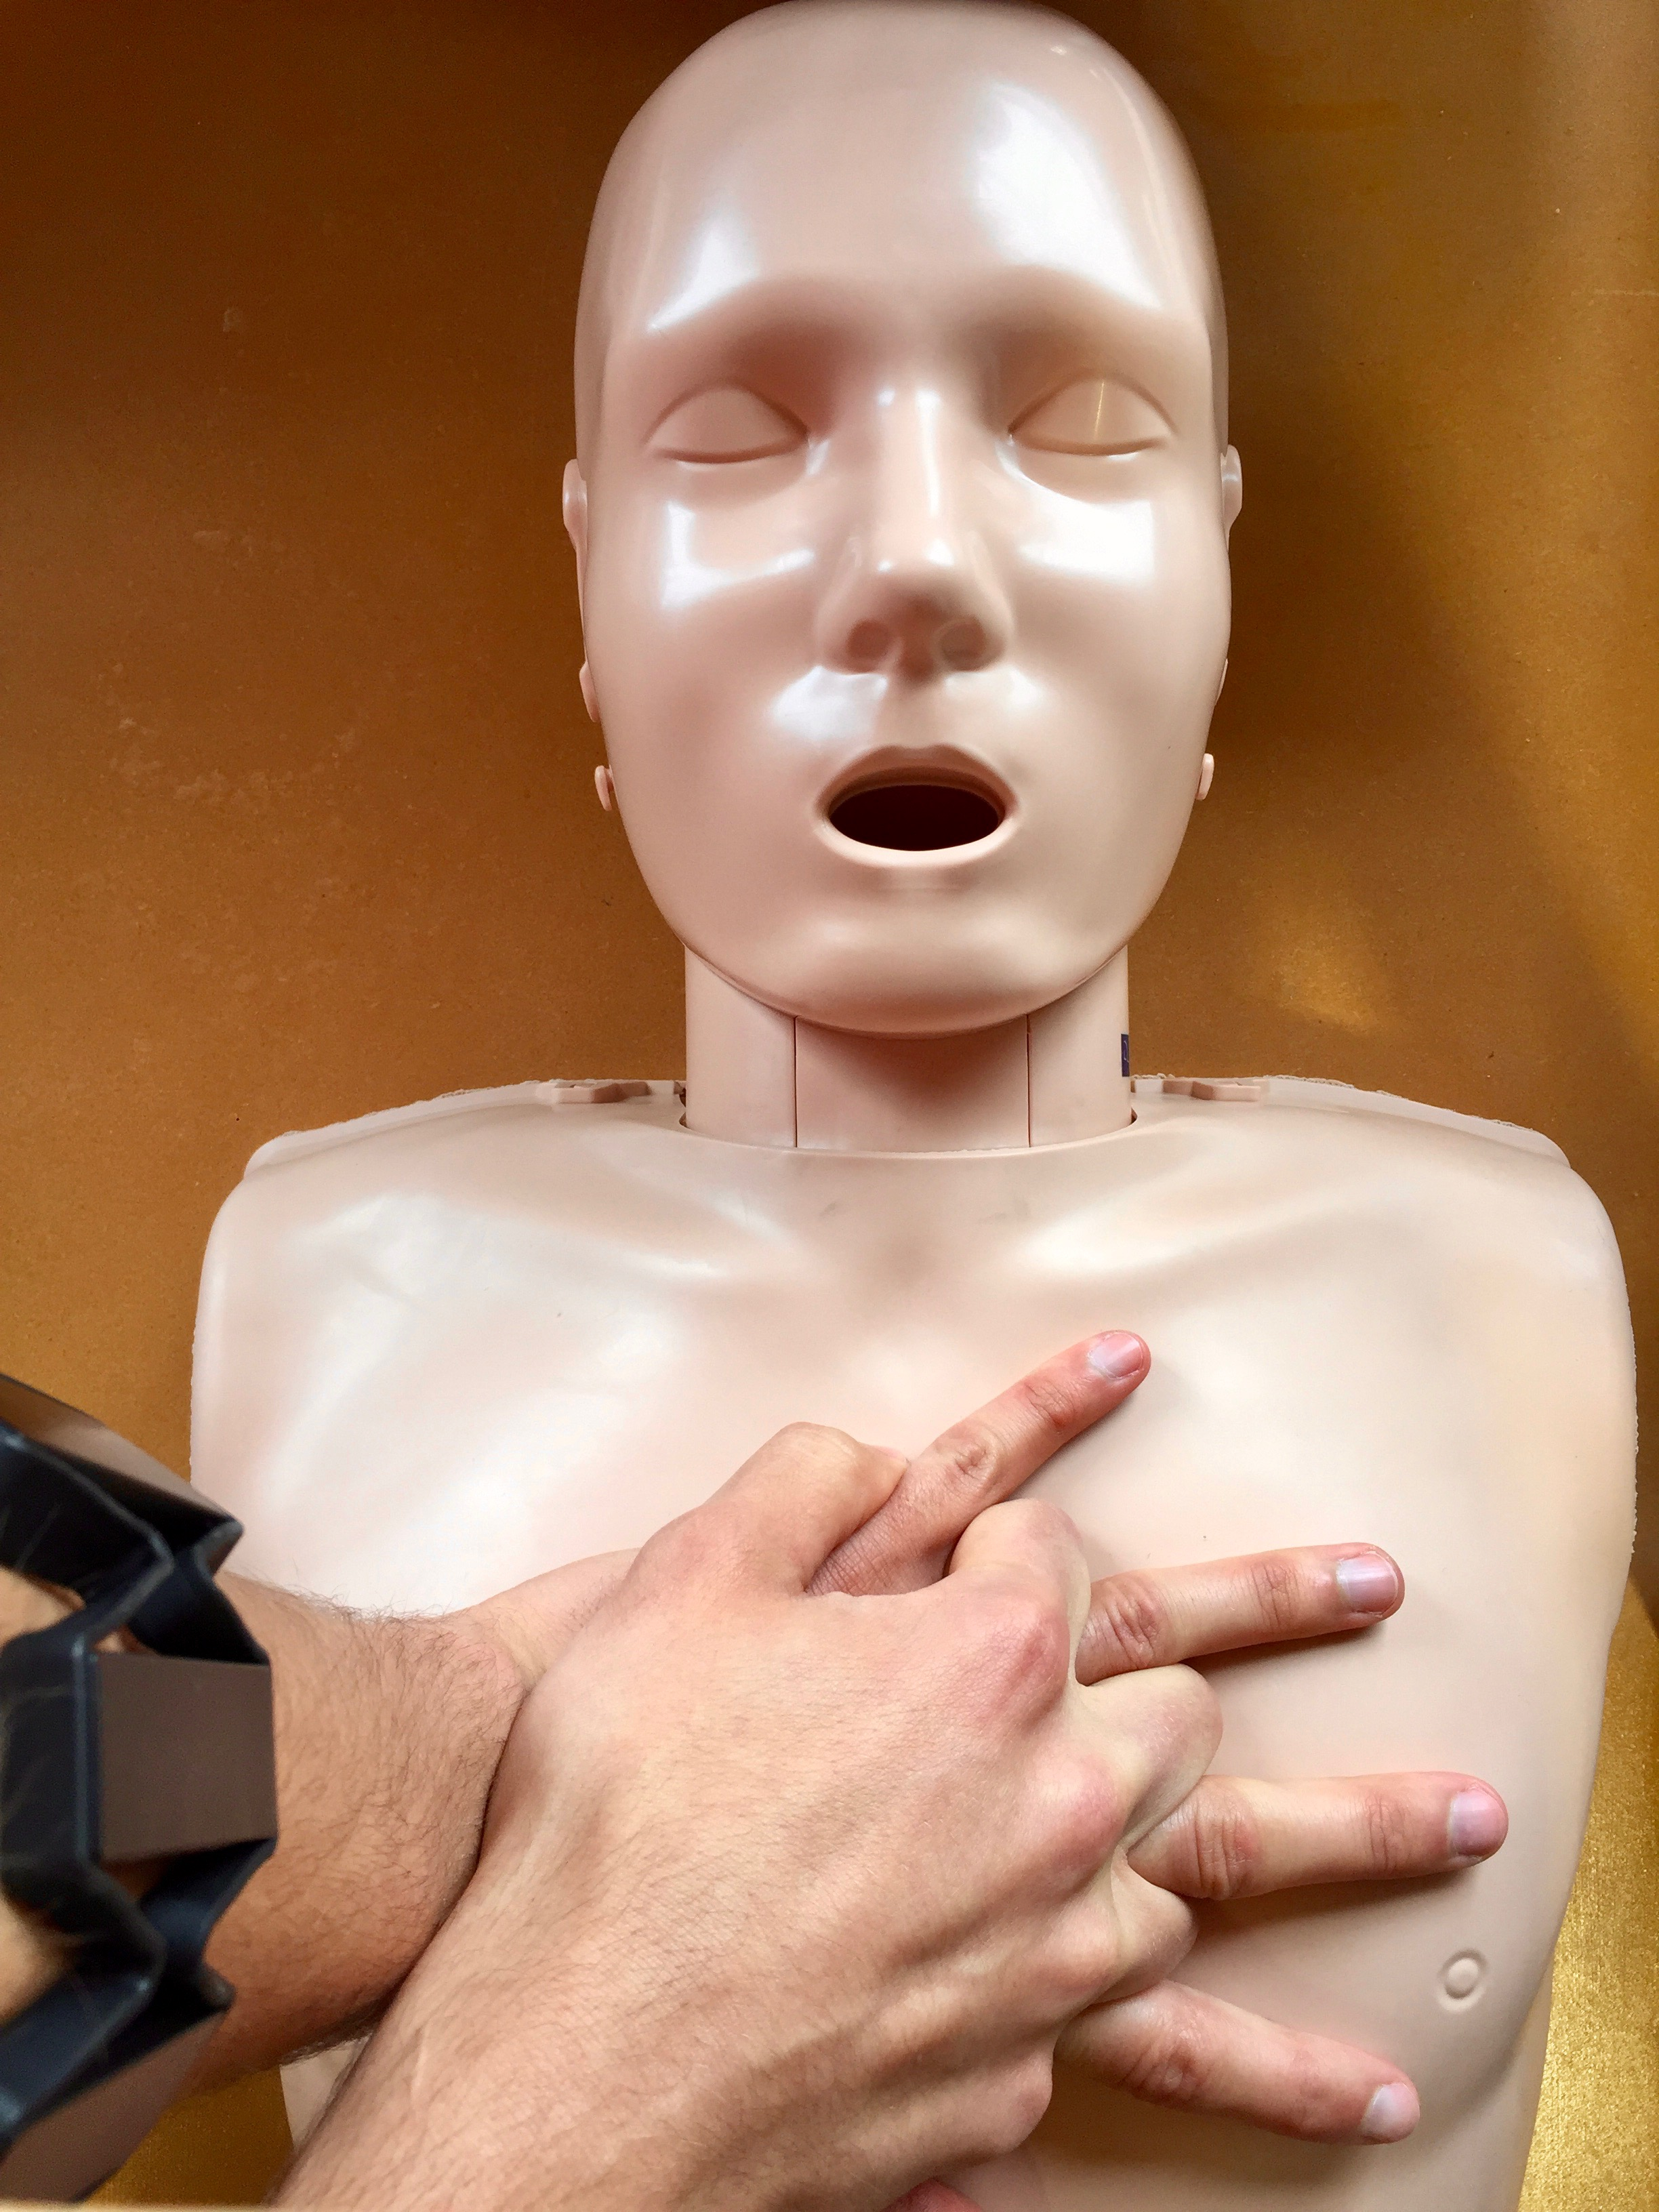
\includegraphics[width=\textwidth]{pictures/cpr}
 		\caption{CPR}
 		\label{fig:cpr}
 	\end{subfigure}
 	~ %add desired spacing between images, e. g. ~, \quad, \qquad, \hfill etc. 
 	%(or a blank line to force the subfigure onto a new line)
 	\begin{subfigure}[b]{0.18\textwidth}
 		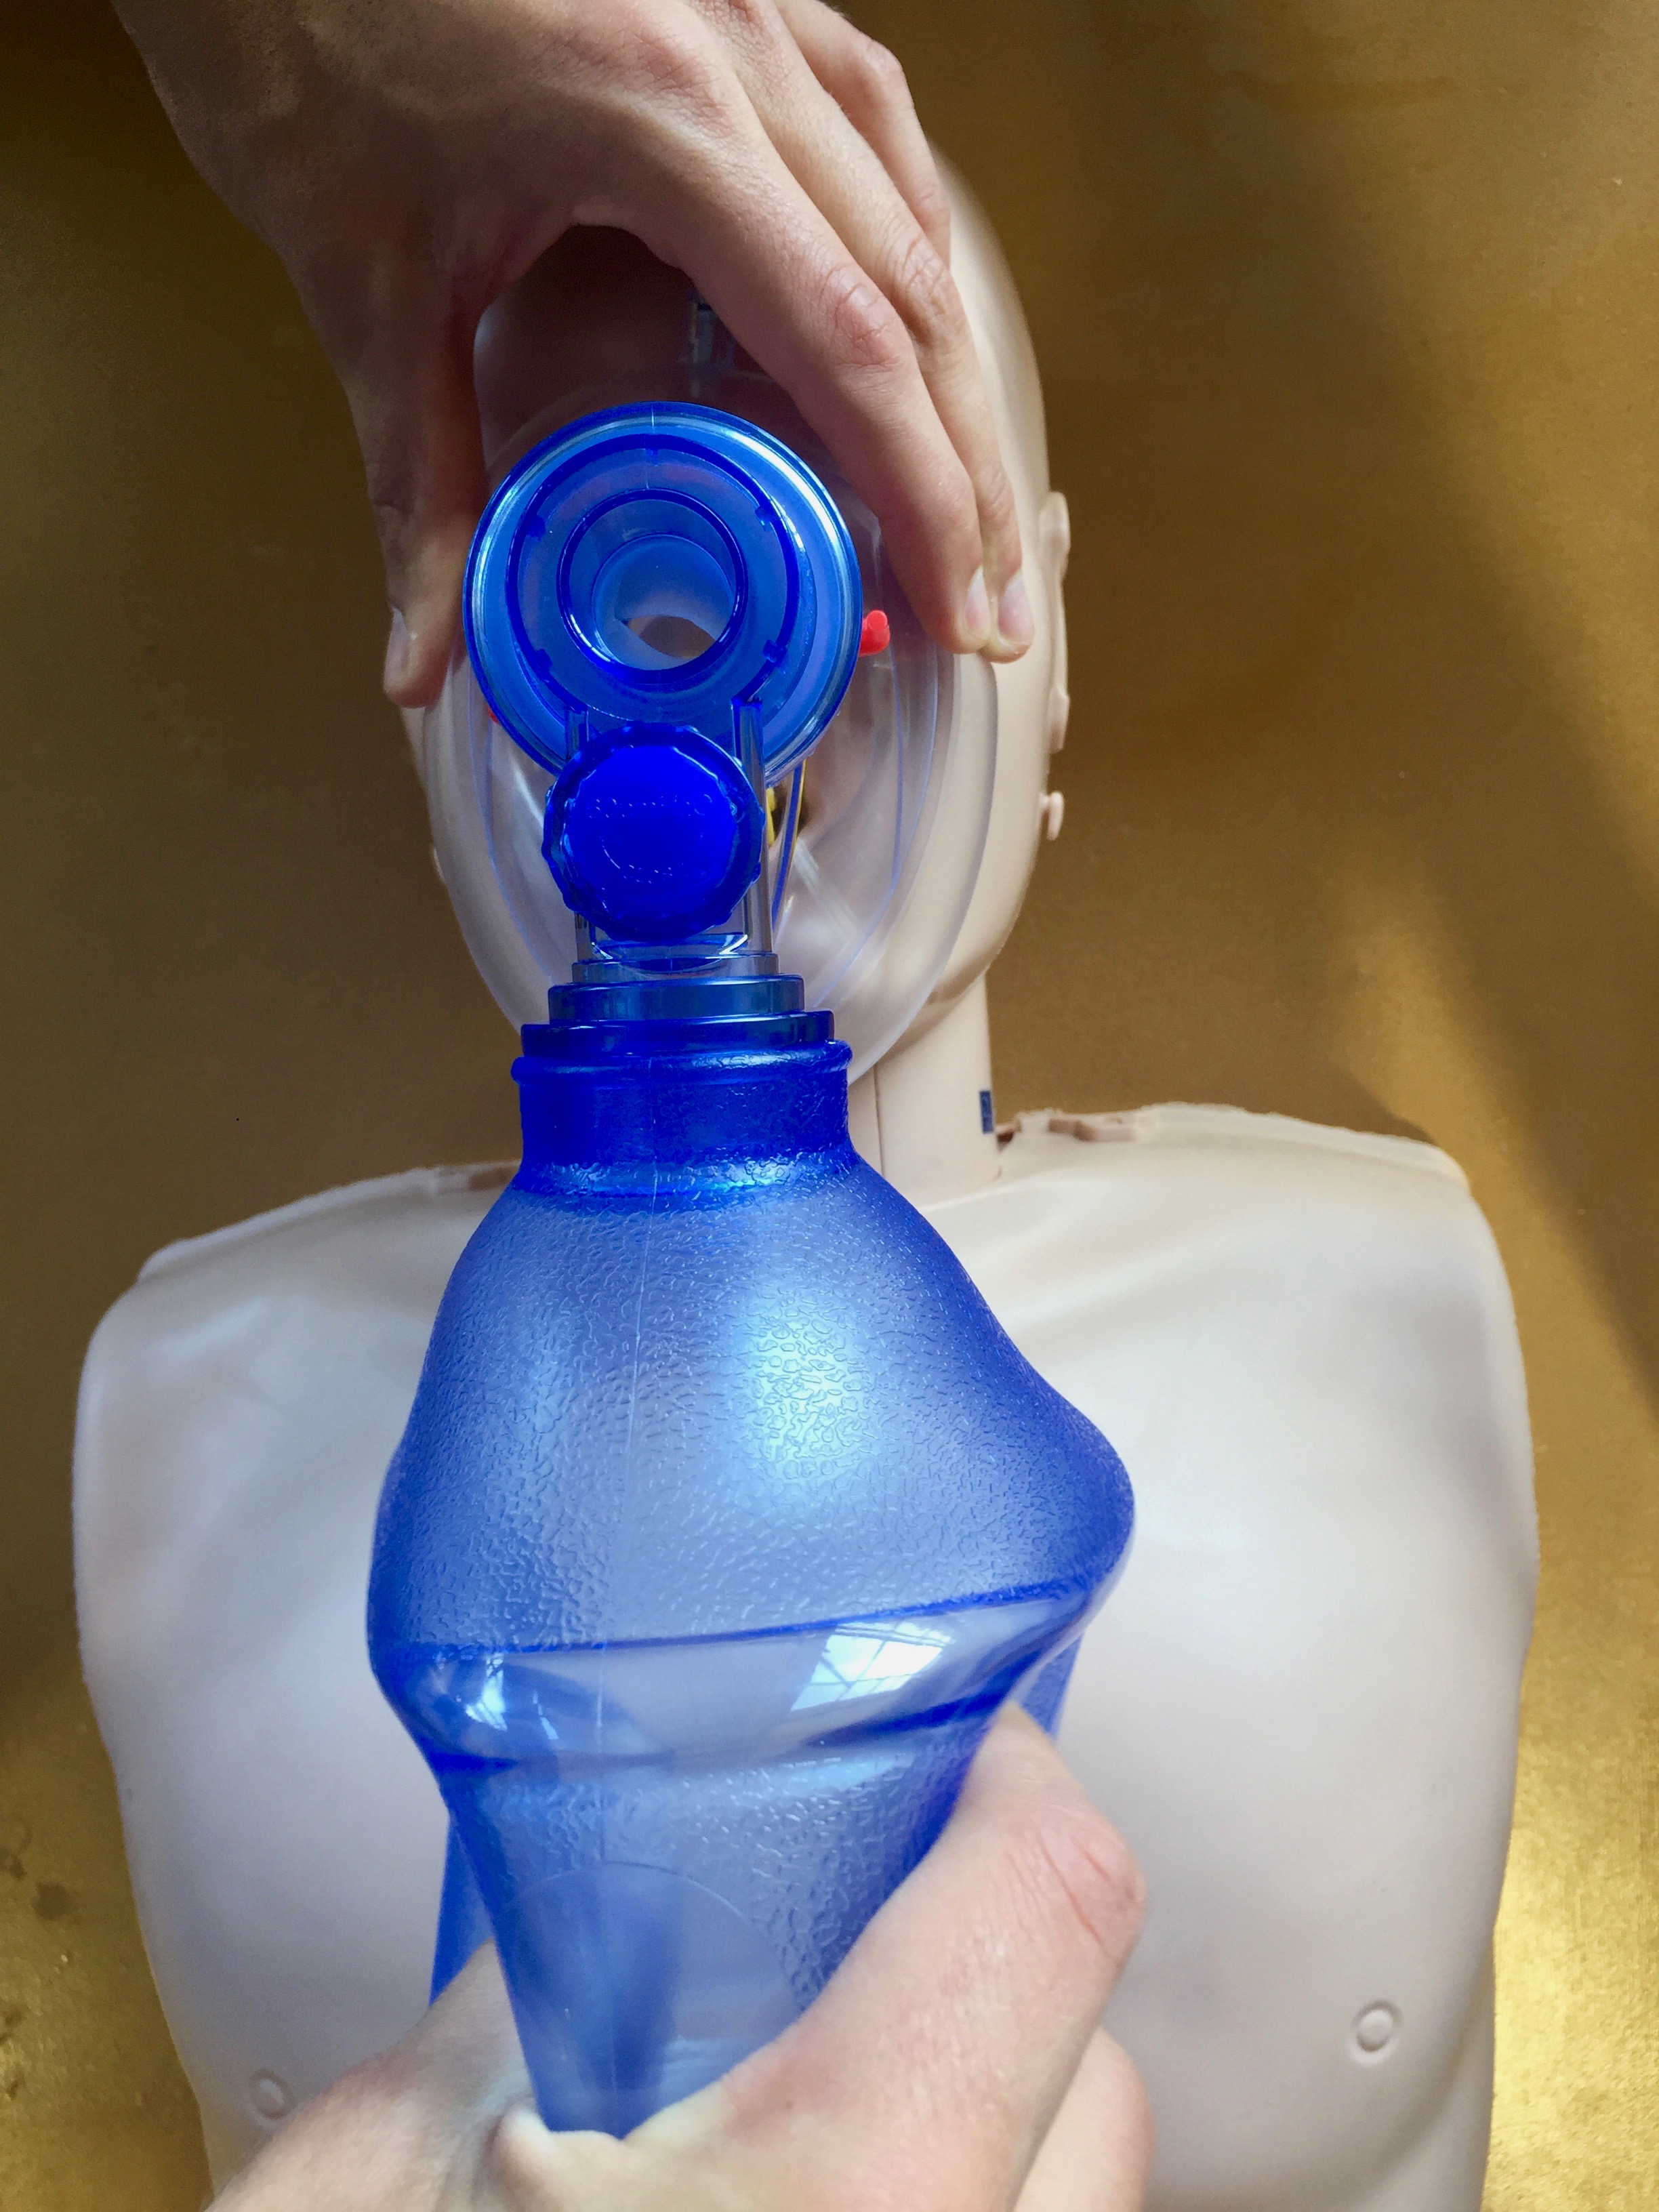
\includegraphics[width=\textwidth]{pictures/bagging}
 		\caption{Bagging}
 		\label{fig:bagging}
 	\end{subfigure}
 	~ %add desired spacing between images, e. g. ~, \quad, \qquad, \hfill etc. 
 	%(or a blank line to force the subfigure onto a new line)
 	\begin{subfigure}[b]{0.18\textwidth}
 		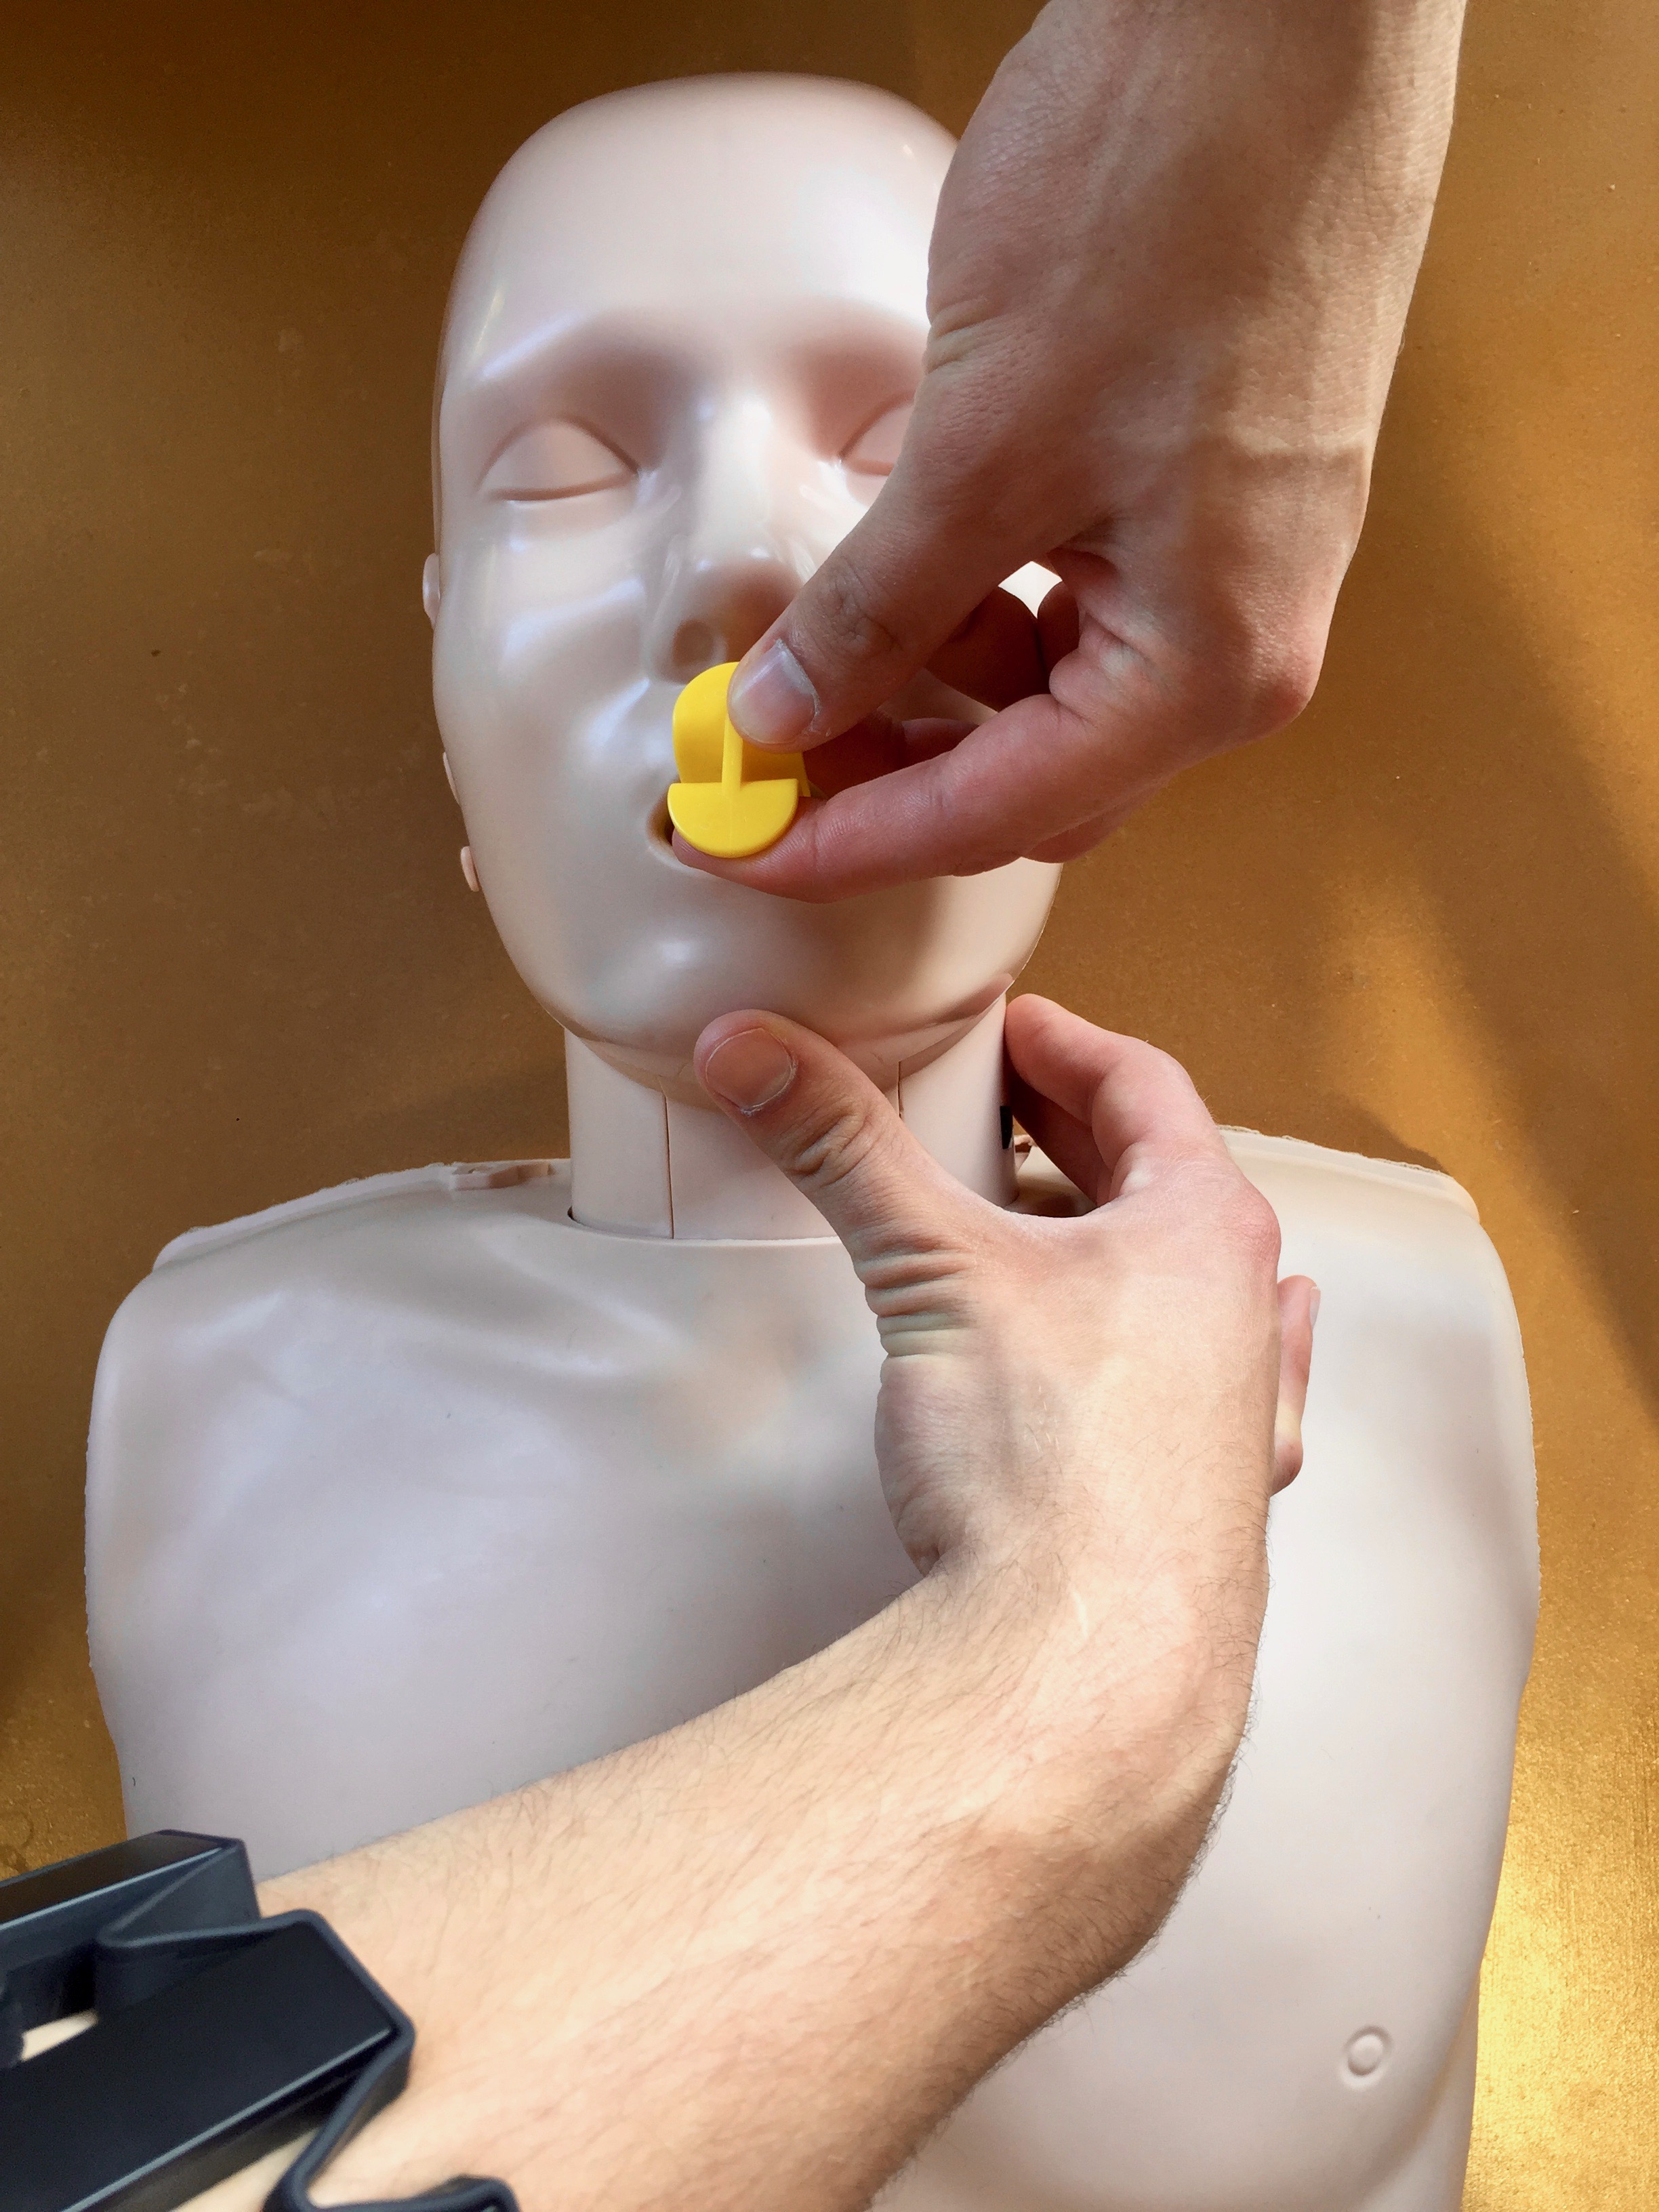
\includegraphics[width=\textwidth]{pictures/oral-airway}
 		\caption{Airway}
 		\label{fig:oral-airway}
 	\end{subfigure}
 	~ %add desired spacing between images, e. g. ~, \quad, \qquad, \hfill etc. 
	 %(or a blank line to force the subfigure onto a new line)
	 \begin{subfigure}[b]{0.18\textwidth}
 		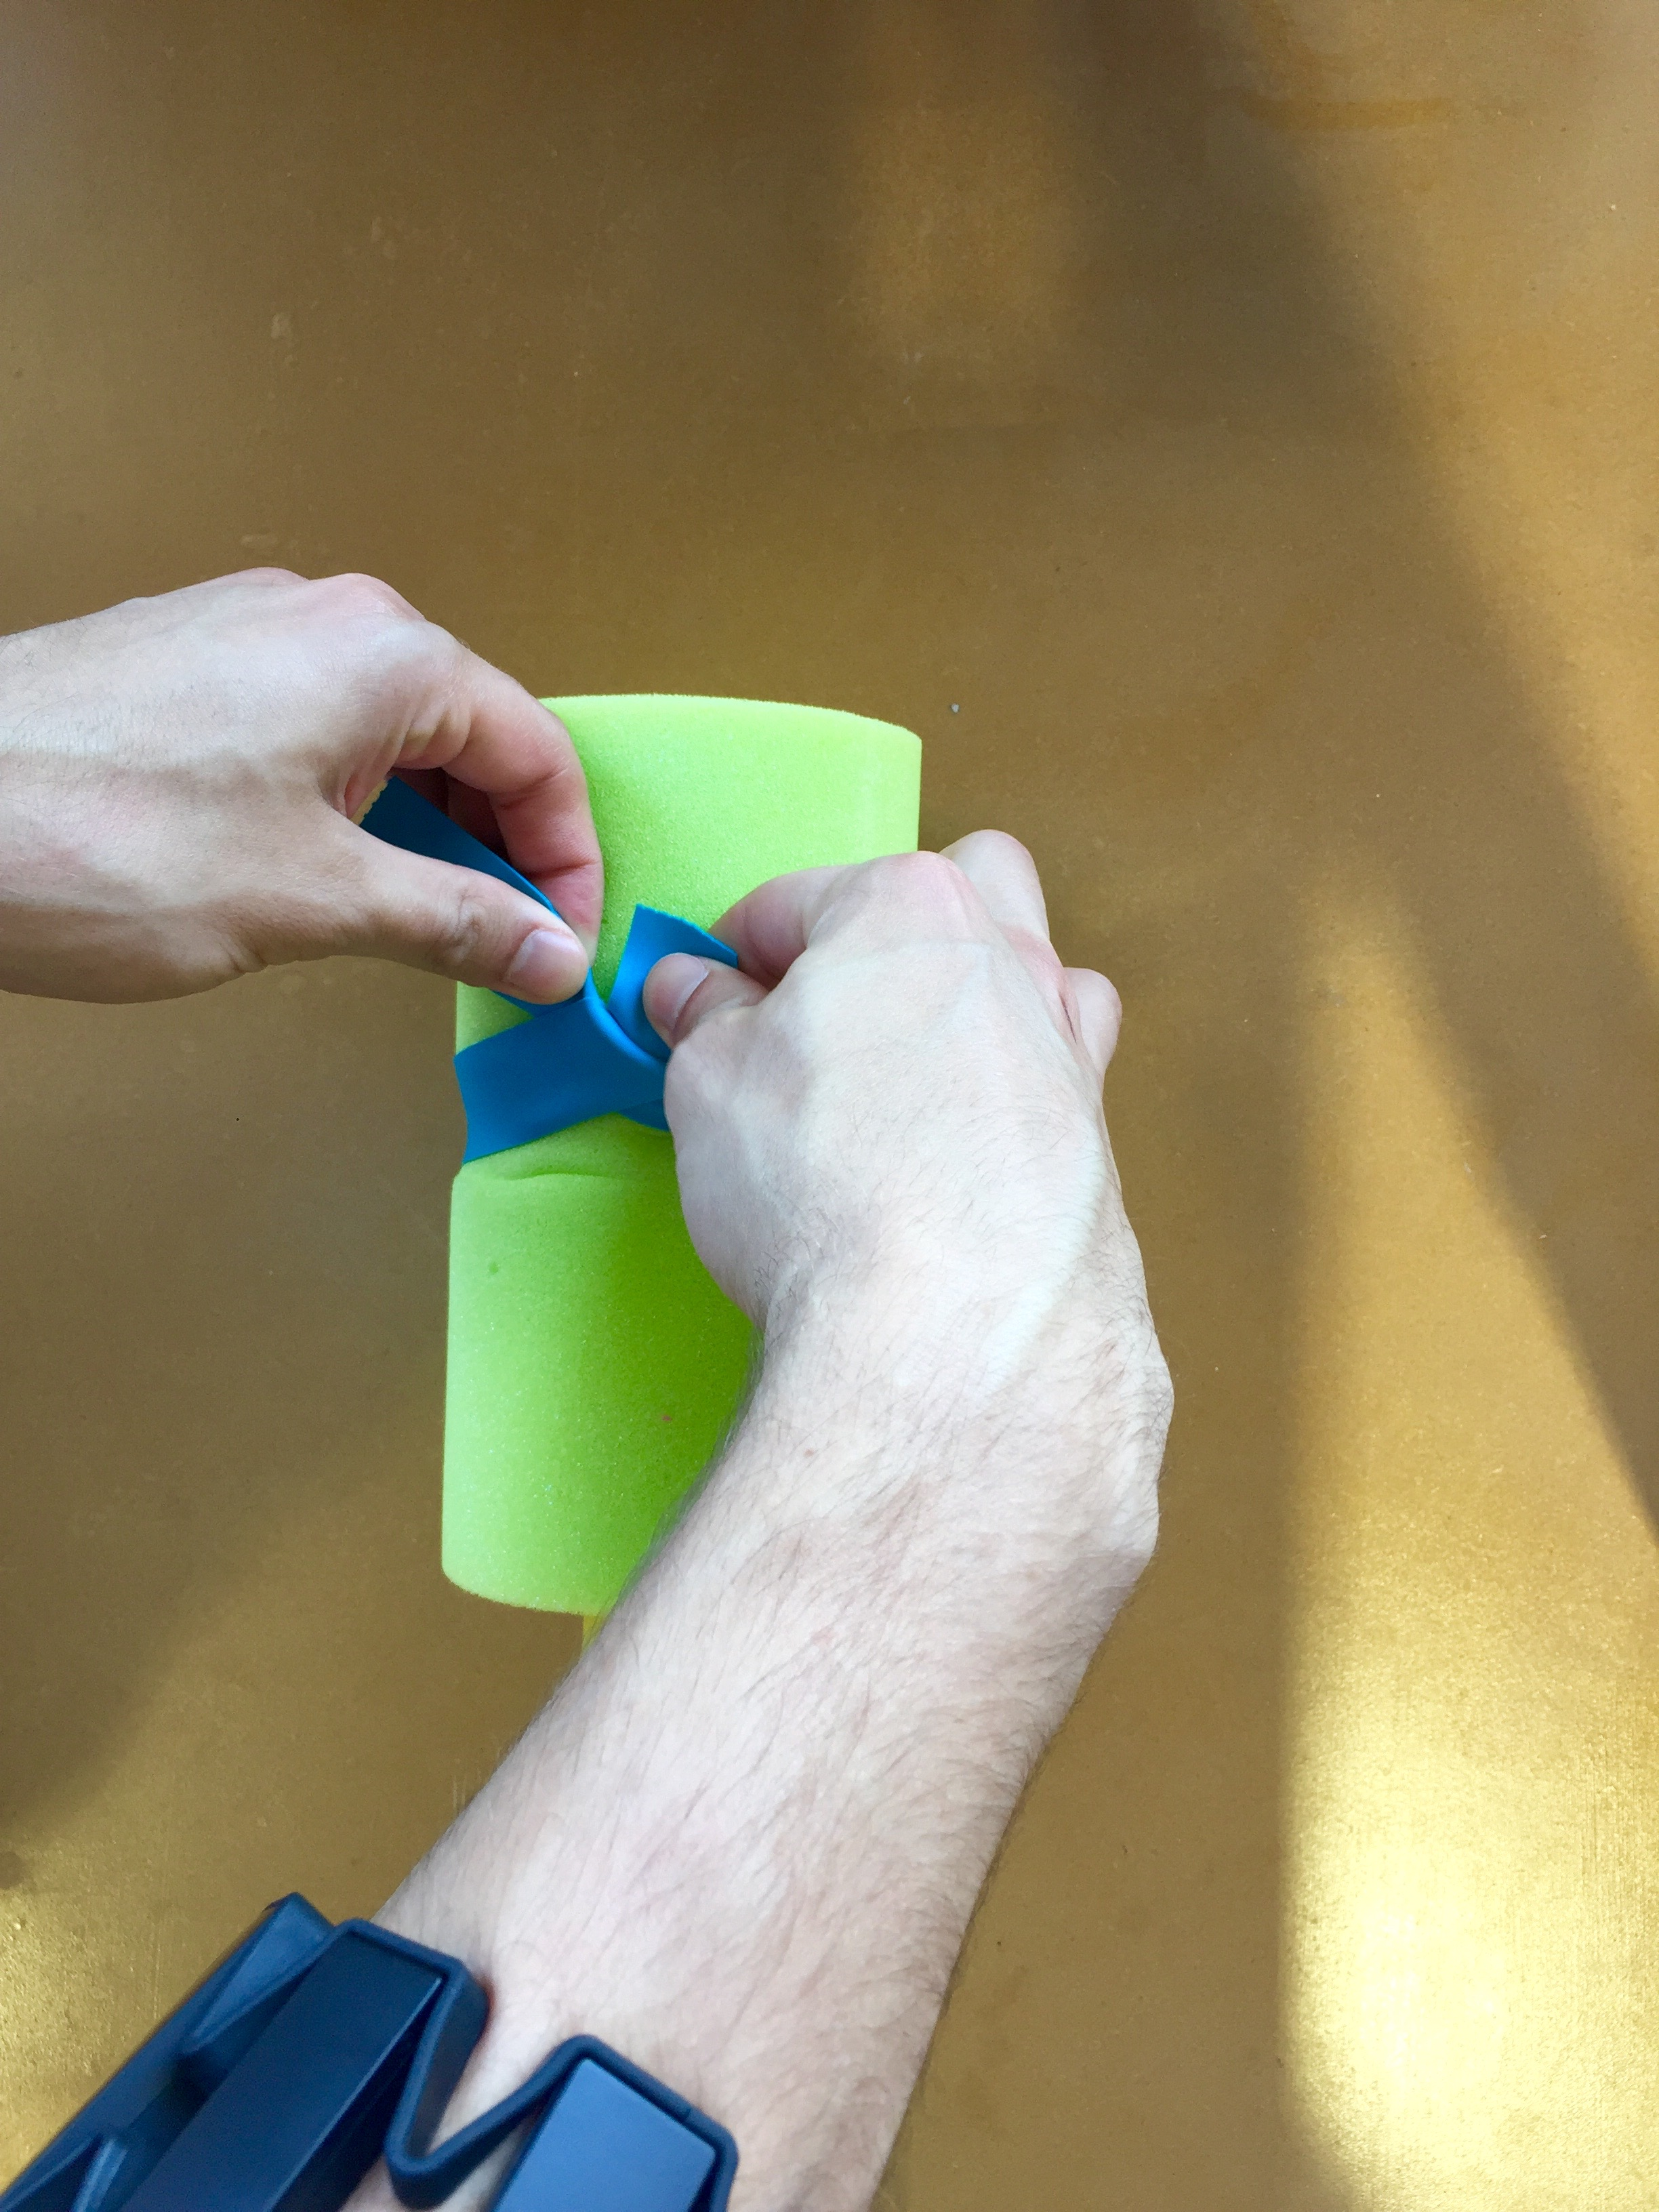
\includegraphics[width=\textwidth]{pictures/tourniquet}
 		\caption{Tourniquet}
 		\label{fig:tourniquet}
 	\end{subfigure}
	~ %add desired spacing between images, e. g. ~, \quad, \qquad, \hfill etc. 
	%(or a blank line to force the subfigure onto a new line)
	\begin{subfigure}[b]{0.18\textwidth}
		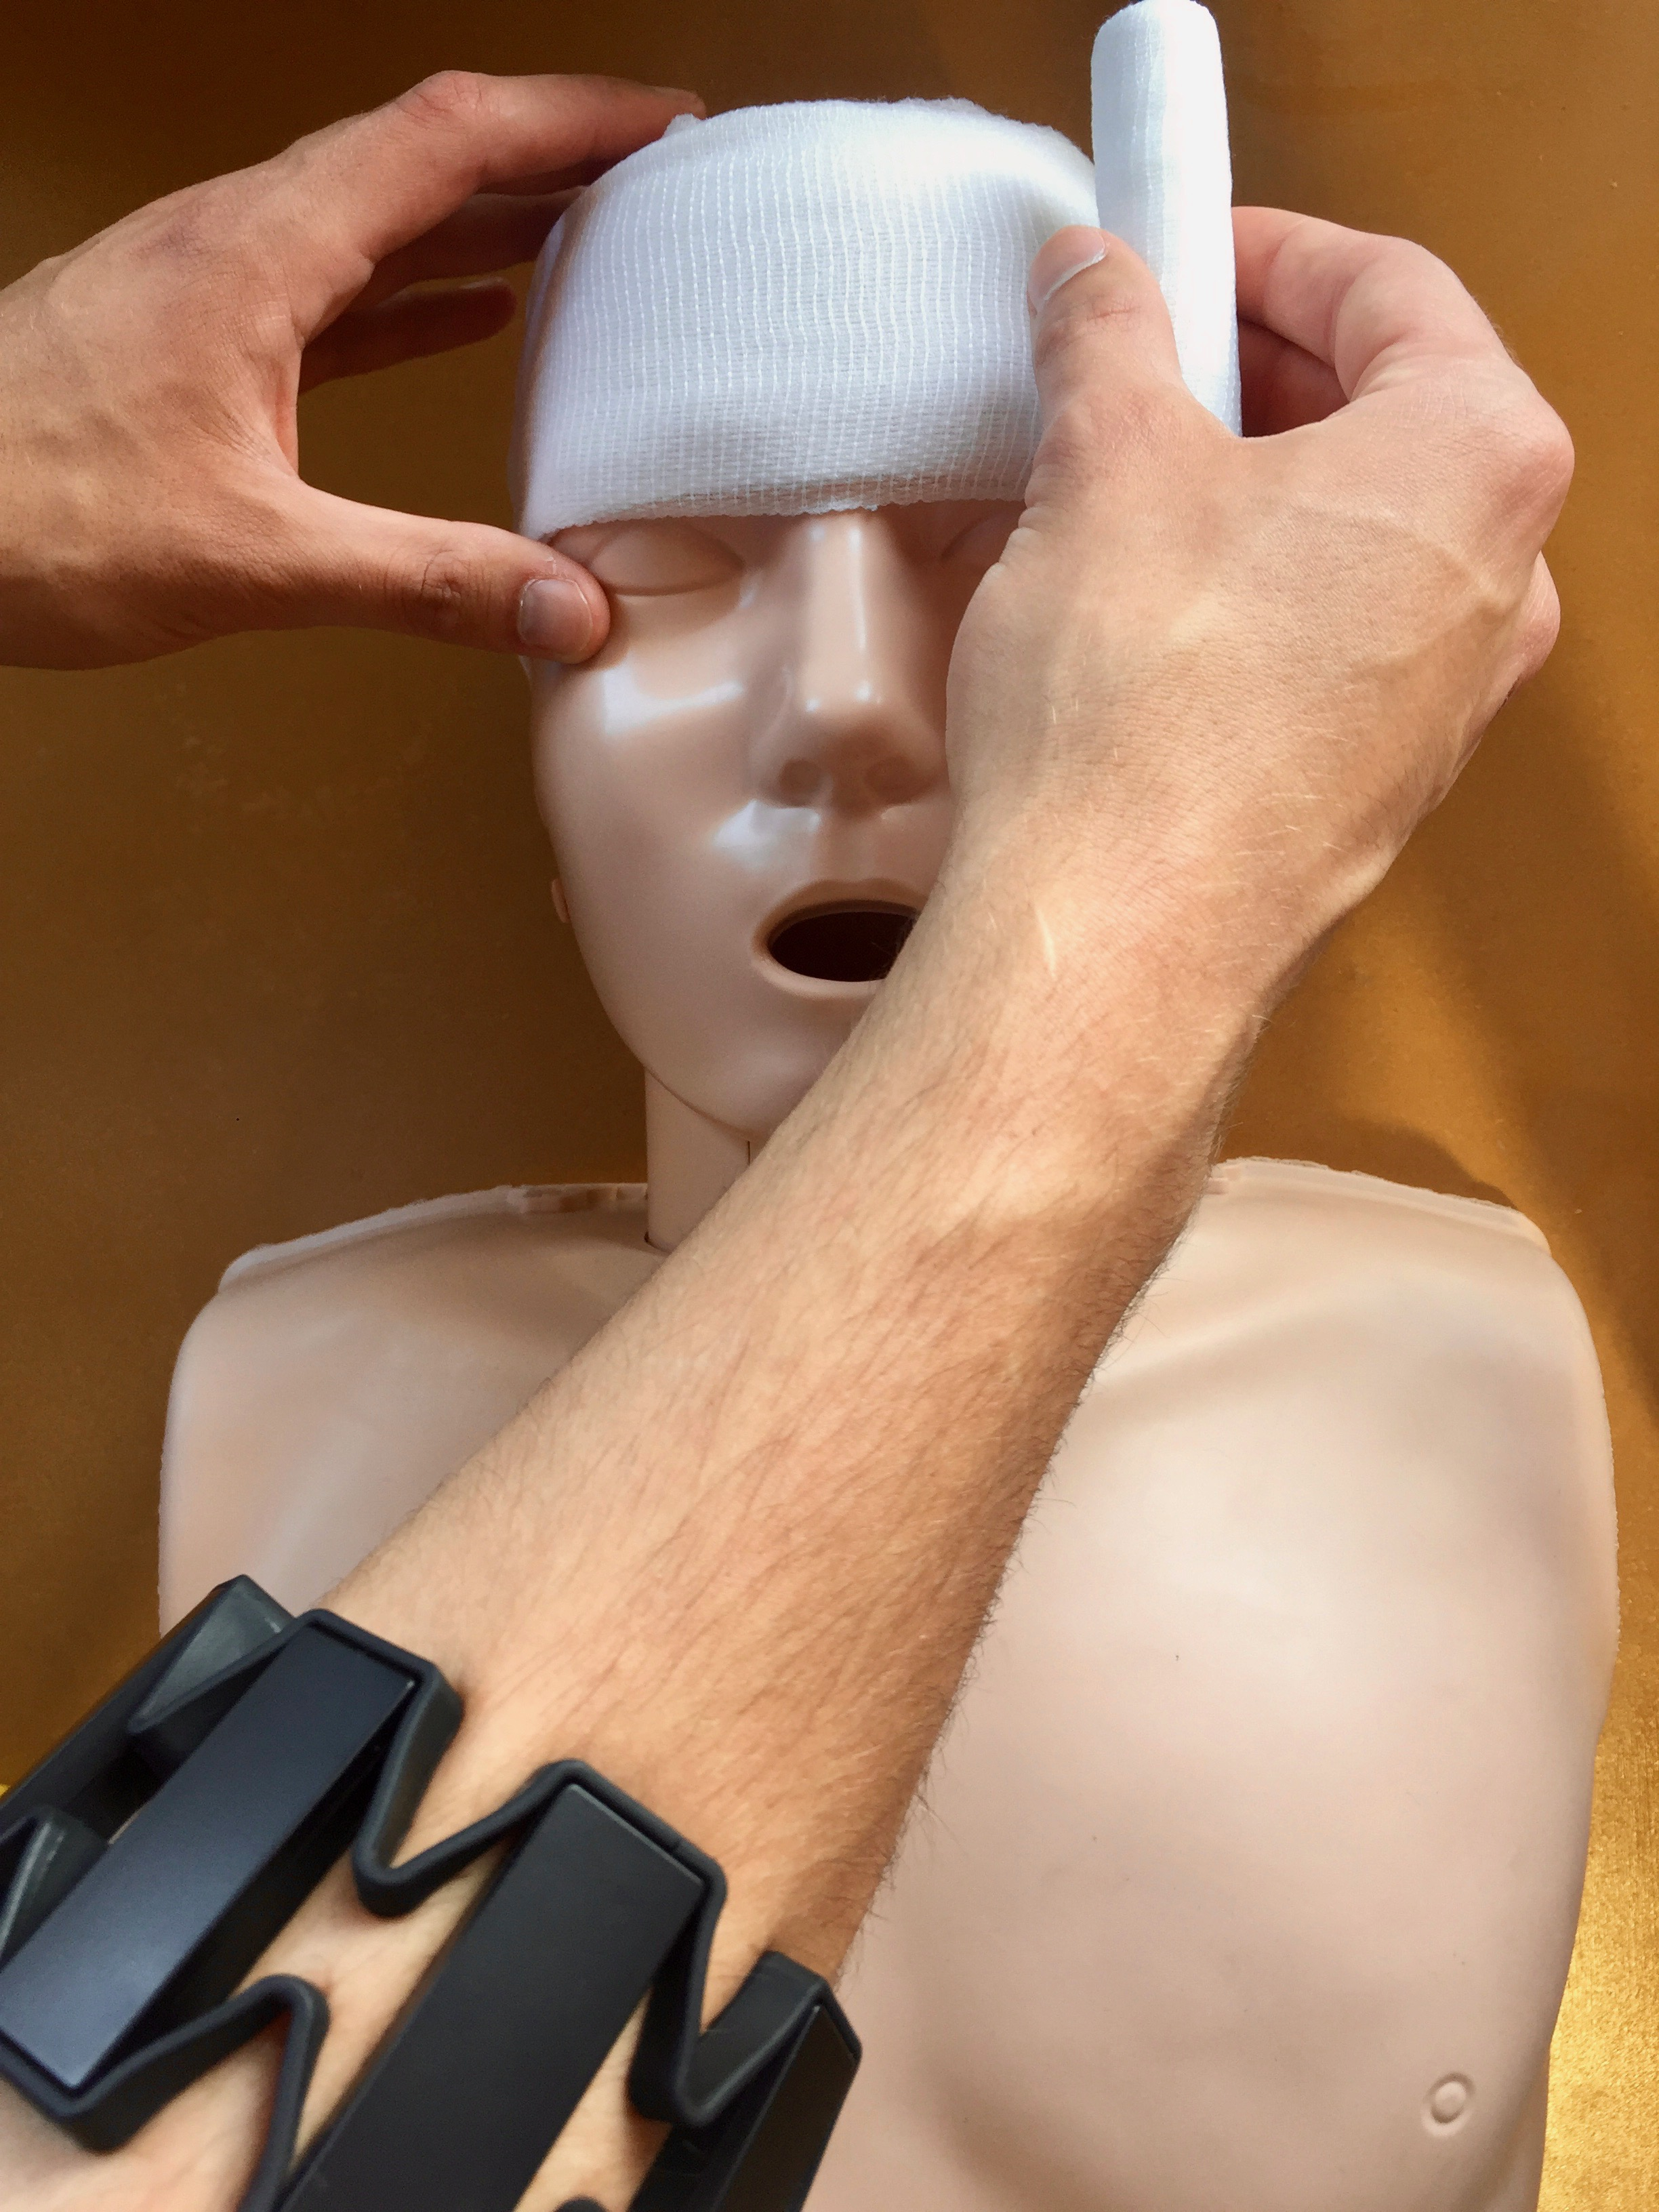
\includegraphics[width=\textwidth]{pictures/wound}
		\caption{Wound}
		\label{fig:wound}
	\end{subfigure}
 	\caption{EMS procedures}
 	\label{fig:EMS-procedures}
\end{figure}
\par CPR is a procedure that is performed on patients with cardiac arrest to preserve brain functionality. Hierarchical Task Analysis of CPR (Table \ref{tab:hta:cpr}) resulted in four sub-tasks, with two ways to perform sub-task number three. The first sub-task for EMS personnel is to lift the patient's chin, then check for breathing. If the patient is not breathing, there are two ways to give breaths: mouth-to-mouth and using a bag-valve-mask. The study uses the bag-valve-mask to ventilate the patient, as the mask is commonly used by EMS personnel. After giving two breaths, 30 compressions are performed. This is repeated until the patient has stabilized. CPR contains 27 anatomical task movements when ventilating using a bag-valve-mask, of which five were determined not to be sensable using the commercial sensors. The Myo is capable of detecting 22 anatomical tasks, 14 more than the other commercial sensors.
\par Bag-Valve-Mask ventilation is a procedure used to artificially breath air into a patient's lungs. Hierarchical Task Analysis of Bag-valve-mask ventilation (Table \ref{tab:hta:bagging}) resulted in four sub-tasks, with two ways to perform sub-task number three. The first sub-task for EMS personnel is to raise the patient until the ear is level with the eternal notch, then the patient's chin is lifted. If the patient is unresponsive an oral airway is placed, otherwise a nasal airway is placed. The study uses oral airways, as the demo mannequin does not feature a nasal canal. Finally the patient is ventilated using the bag-valve-mask. A total of 26 anatomical task movements were found, of which one was determined to not be sensable using the commercial sensors. The Myo is capable of detecting 25 anatomical tasks, eight more than the other commercial sensors.
\par Placing an intravenous tourniquet is a procedure to highlight veins by constricting blood flow. Hierarchical Task Analysis of placing an intravenous tourniquet (Table \ref{tab:hta:tourniquet}) resulted in two different sub-tasks. At first an EMS personnel has to grab a tourniquet. Then the tourniquet is applied by tying it around the body part. A total of seven anatomical task movements were found, of which all were determined to be sensable using the Myo, two more than the other commercial sensors.
\par Wrapping a wound is a procedure to stop bleeding of an open wound. Hierarchical Task Analysis of wrapping a wound (Table \ref{tab:hta:wound}) resulted in two sub-task. At first an EMS personnel has to grab a the pressure dressing. Then the pressure dressing is placed on the wound and wrapped around it. A total of five anatomical task movements were found, of which all were determined to be sensable using the Myo, one more than the other commercial sensors.
\newcommand*\rot{\multicolumn{1}{R{45}{1em}}}
\begin{table}[htbp]
	\begin{tabular}{lrrrrrrrrr}
		\textbf{Task} & \rot{\textbf{\# Sub-Tasks}} & \rot{\textbf{\# Multi-Hand Sub-Tasks}} & \rot{\textbf{\# Task Movements}} & \rot{\textbf{\# Unsensed Task Movements}} & \rot{\textbf{\% Sensed} Apple Watch} & \rot{\textbf{\% Sensed} MYO} & \rot{\textbf{\% Sensed} Empatic E4} & \rot{\textbf{\% Sensed} Garmin Forerunner} & \rot{\textbf{\% Sensed} Bioharness BT} \\
		\midrule
		\textbf{CPR} & 5     & 4     & 36    & 7     & 39\%  & 61\%  & 39\%  & 39\%  & 19\% \\
		\textbf{Bagging} & 5     & 2     & 27    & 1     & 48\%  & 96\%  & 48\%  & 48\%  & 0\% \\
		\textbf{Oral Airway} & 4     & 1     & 16    & 0     & 50\%  & 100\% & 50\%  & 50\%  & 0\% \\
		\textbf{Place a Tourniquet} & 2     & 2     & 7    & 0     & 71\%  & 100\% & 71\%  & 71\%  & 0\% \\
		\textbf{Wrapping a wound} & 2     & 3     & 24    & 1     & 58\%  & 96\%  & 58\%  & 58\%  & 0\% \\
	\end{tabular}
	\caption{Hierarchical Task Analysis: Overview}
	\label{tab:hta:overview}
\end{table}
\par The Myo was chosen as the wireless sensor for the study due to its capability to sense most of the anatomical movement. Two Myo devices expands the coverage for data collection to both arms, which is useful in detecting multi-hand tasks.
\par Task recognition results in higher accuracy when each procedure has unique movements, as there are significant changes in patterns \cite{5370804}. The five procedures include two unique sub-tasks: compression for CPR, and ventilating the patient for bag-valve-mask ventilation. There are several overlapping sub-tasks:
\begin{itemize}
	\item \textbf{squeezing a bag} for CPR, and bag-valve-mask ventilation;
	\item \textbf{lifting a patient's chin} for bag-valve-mask ventilation, and placing an oral airway;
	\item \textbf{moving the valve mask into position} for CPR, and bag-valve-mask ventilation;
	\item \textbf{grabbing the valve mask} for CPR, and bag-valve-mask ventilation; raising the patient for bag-valve-mask ventilation, and placing an oral airway;
	\item \textbf{placing an oral airway (oropharyngeal)} for bag-valve-mask ventilation, and placing an oral airway;
\end{itemize}
Overlapping sub-tasks have to be treated with caution as they solely can not directly identify a procedure. The unique sub-tasks may be clear indicators that the procedure associated with that sub-task is being performed, while overlapping sub-tasks are not clear indicators. Therefore, when a unique sub-task is detected it is safe to reliably infer the associated procedure, while an overlapping sub-task requires further sub-tasks in the sequence.

\section{Algorithm}
\label{sec:Approach:Algorithm}
The algorithm to recognize procedures performed by EMS personnel inside an ambulance relies on acceleration, gyroscope, and EMG data. Human activity recognition algorithm have been proven to accuracy detect activities when using acceleration, gyroscope, and EMG data.

\subsection{Data Acquisition}
Acceleration, gryoscope, and EMG data are acquired through the Myo armband. The Myo armband is created by Thalmic Labs, Inc. and includes an EMG sensor, triaxial accelerometer, a triaxial gyroscope, and triaxial magnetometer. The data from the magnetometer is not used in the algorithm, due to its susceptibility to environmental noise \cite{Ahmad2013}. Acceleration and gyroscope data is available at 50Hz, while EMG data is available at 200Hz. The EMG data has eight channels with 8bits of resolution for each channel. The accelerometer data consists of $x$, $y$, and $z$ values, and the gyroscope data has $roll$, $pitch$, and $yaw$ (Figure \ref{fig:myo}). The Myo's $z$ axis is perpendicular to the floor, while the $x$ and $y$ axis are in the plane relative to the floor. The Myo's $pitch$ axis is rotating the arm up and down, the $yaw$ axis is rotating the arm side to side, and the $roll$ axis is rotating the arm along itself. Finally, the Myo has an output for proprietary hand gesture recognition, which is used as a feature for the algorithm: pinch, fist, open, wave in, and wave out.

\begin{figure}
	\centering
	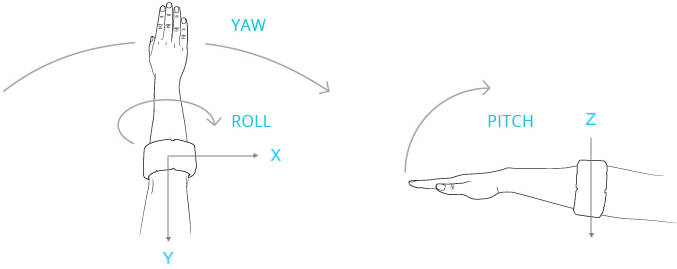
\includegraphics[width=0.7\linewidth]{pictures/myo}
	\caption{Myo Reference Frame}
	\label{fig:myo}
\end{figure}


\subsection{Data Processing}
\label{sec:Approach:Data-Processing}
The data from the acceleration, gyroscope, and EMG sensor needs to be processed in order to reduce noise and motion artifacts. Accelerometer and gyroscope data is smoothed using a $4^{th}$ order Butterworth band-pass filter with cut-off frequencies at 0.2Hz and 15Hz \cite{1419604}. The EMG data is high-pass filtered at 20Hz to reduce motion artifacts as recommended in previous works \cite{DeLuca2010}. The data is retrieved at the frequency of the EMG sensor at 200Hz, while the accelerometer and gryoscope data is updated at 50Hz. Retrieving data from all sensors at the highest frequency prevents empty data cells, which can cause problems when extracting features.

\subsection{Feature Extraction}
\label{sec:Approach:Feature-Extraction}
Human activity recognition systems take features extracted from processed data as input. The features are calculated through the use of a sliding window. Due to time it takes to perform different anatomical movements, the window size will have a length of 2s. The window will have a 50\% overlap, which has been proven sufficient in related work \cite{Wannenburg2016}.
\begin{table}[h]
	\centering
	\begin{tabular}{c|l|l}
		& \multicolumn{1}{l|}{Domain} & \multicolumn{1}{c}{Features} \\
		\hline
		\parbox[t]{2mm}{\multirow{3}{*}{\rotatebox[origin=c]{90}{IMU}}} & Time & Mean\\
		&& Standard deviation\\
		&& Signal Magnitude Area\\
		\hline
		\parbox[t]{2mm}{\multirow{3}{*}{\rotatebox[origin=c]{90}{EMG}}} & Time & Mean\\
		&& Signal Magnitude Area \\
		&& Root Mean Squared \\
		& Frequency & Power Spectral Density \\
	\end{tabular}
	\caption{Features for the Machine Learning algorithm}
	\label{tab:features}
\end{table}
\emph{Mean acceleration} is calculated by excluding the highest and lowest 10\% of the data, taking the sum of each of the three accelerometer axes and dividing by the number of values \cite{Totty2017}. Excluding the outliers removes any spikes that may occur due to collisions.
\begin{align*}
mean\_acceleration_{axis} = \sum_{i=1}^{N}acceleration_{axis}\\
axis = \{x,y,z\}, N = \text{number of acceleration values}
\end{align*}
The mean acceleration feature was chosen to represent the quantity of motion \cite{Arif2015}. \emph{Acceleration signal magnitude area} is computed by dividing the numerically-integrated area under the curve by the duration of the signal \cite{Totty2017}.
$$ signal\_magnitude\_area\_acceleration_{axis}= \frac{1}{T}\int_{0}^{T}(|a_x|+|a_y|+|a_z|)dt$$
The signal magnitude area of the acceleration feature was chosen, because it represents the gross motion of movements and the energy expenditure \cite{Jeran2016}. \emph{Mean angular rate of change} is calculated by taking the sum of the three gyroscope axes \cite{Totty2017}. The mean rate of change feature was chosen, because it represents the quantity of rotation. \emph{Angular rate of change signal magnitude area} is calculated by dividing the numerically-integrated area under the curve by the duration of the signal \cite{Totty2017}.
$$ g_{sma} = \frac{1}{T}\int_{0}^{T}(|\theta_x|+|\theta_y|+|\theta_z|)dt$$
The angular rate of change signal magnitude area feature was chosen, because it represents the gross rotation of movements.
\emph{Mean muscle activation} is calculated by taking the sum of the eight EMG channels. \emph{Muscle activation signal magnitude area} is calculated by dividing the numerically-integrated area under the curve by the duration of the EMG signal.
$$ e_{sma} = \frac{1}{T}\int_{0}^{T}(|e1|+|e2|+|e3|+|e4|+|e5|+|e6|+|e7|+|e8|)dt$$
The mean muscle activation feature was chosen, because it represents the quantity of muscle movement.
\emph{Muscle activation root mean squared} is calculated for each of the eight EMG channels and then averaged.
$$ e1_{rms} = \sqrt{\frac{1}{n}(e1_1^2+e1_2^2+e1_3^2+\dots+e1_n^2)} $$
$$ e2_{rms} = \sqrt{\frac{1}{n}(e2_1^2+e2_2^2+e2_3^2+\dots+e2_n^2)} $$
$$ \dots $$
$$ f_{rms} = \frac{1}{8}\sum_{i=1}^{8}ei_{rms} $$
Root mean squared is proven to be the gold standard for EMG-force analysis \cite{KALLENBERG2008780}. The root mean squared value represents physiological activity during contraction of the muscle \cite{Totty2017}.
\emph{EMG Fast Fourier transformation} is applied to each EMG channel to transform the signal from the time domain into the frequency domain. The frequency spectrum can be used to detect muscle fatigue, force production and muscle fiber signal conduction velocity \cite{Gler2005}.
\subsection{Machine Learning}
\label{sec:Approach:Machine-Learning}
Two machine learning approaches are evaluated for their accuracy in detecting five common procedures performed by EMS personnel. The first approach is taking the extracted features of every procedure and training a Support Vector Machine (SVM), decision-tree, and $k$-NN machine learning algorithm. SVMs work by constructing hyperplanes between classes. SVMs use different kernel to define the hyperplane, such as: linear, polynomial, and Gaussian radial basis function. A decision-tree is a graph in which each node is a test of comparing data values to a condition, each branch is the result of the test, and each leaf is the class label. Finally, $k$-NN is a algorithm where the inputs are the $k$ closest neighbors of the data point. The algorithm counts the class label of each label and determines the label of the data point using majority voting. The second approach is using the fine-grained movements sequence of a procedure and training a separate Hidden Markov Model (HMM) for each procedure. The states for the HMM are the sub-tasks of the procedure. The Baum-Welch algorithm is used in combination with the Forward-Backward algorithm to train the HMM parameters.

\section{Experimental Design}
\label{sec:Experimental-Design}
A machine learning algorithm needs data from different people performing all five procedures a number of times in order to be trained. The following chapter describes a study design to collect data from participants for the automatic recognition system. 

\subsection{Data Collection}
\label{sec:Experimental-Design:Data-Collection}
The study was designed to be within-subjects and consists of two questionnaires, training, and data collection. The first questionnaire asks for the participants demographics. The second questionnaire evaluates the participants fatigueness, which may effect the data collection. The study is split into three days and structured as follows:
\begin{enumerate}
	\item \textbf{Day 1} (1 hour): First, the participant was asked to sign the consent form. Then, after a brief introduction to the experiment, the participant was fitted with two Myos on each of his or her arms. Next, the participant was asked to complete the demographic questionnaire, and the fatigue questionnaire. For the remainder of the time, the participant was trained in the five medical procedures: CPR, wrapping a wound, tying a tourniquet, placing an oral airway, and bagging.
	\item \textbf{Day 2} (1 hour): After the participant was fitted with two Myos on each of his or her arms, he or she completed a fatigue questionnaire. For the remainder of the time, the participant was trained in the five medical procedures.
	\item \textbf{Day 3} (1 hour): After the participant was fitted with two Myos on each of his or her arms, he or she completed the fatigue questionnaire. For the first 15 mins, the participant was reminded of the training in the five medical procedures.
	After a five minute break the participant was asked to complete all five procedures for a minute each with 5 minute breaks in between each procedure. Finally the participant was asked to do four rounds of completing all five procedures in a sequence, with a 5 minute break between each round.
\end{enumerate}

\subsection{Research Questions}
\label{sec:Data-Collection:Research-Questions}
The evaluation of the automatic recognition system focuses on the accuracy of the machine learning algorithm, in order to evaluate two hypotheses:
\begin{itemize}
	\item $H_1$: Recognition of CPR and Bag-valve-mask ventilation will have the highest accuracy.
	\item $H_2$: The recognition of a procedure through the sequence of fine-grained movements using a Hidden Markov Model is more accurate than detecting through training coarse-grained movement models.
\end{itemize}

\subsection{Participant Demographics}
\label{sec:Data-Collection:Participant-Demographics}